\chapter{Physics: Quantum Field Theories}

The Standard Model (SM) of particle physics classifies all known
\index{particle!elementary}\index{Standard Model}
{\it elementary particles}, i.e. particles with no known substructure,
and describes three fundamental forces:\index{force!fundamental} the electromagnetic,
weak, and strong forces. Elementary particles can be divided into
\index{particle!matter}
{\it matter particles} (quarks and leptons); {\it gauge bosons}, which mediate
\index{boson!scalar}\index{boson!gauge}
the three aforementioned forces; and a {\it scalar boson}, the Higgs boson,
whose field interacts directly with elementary particles that thereby
acquire their mass. For each particle there exists a corresponding
antiparticle; sometimes a particle is its own antiparticle.
Figure~\ref{fig:SM} gives a schematic overview of the SM.

\begin{figure}
  \centering
  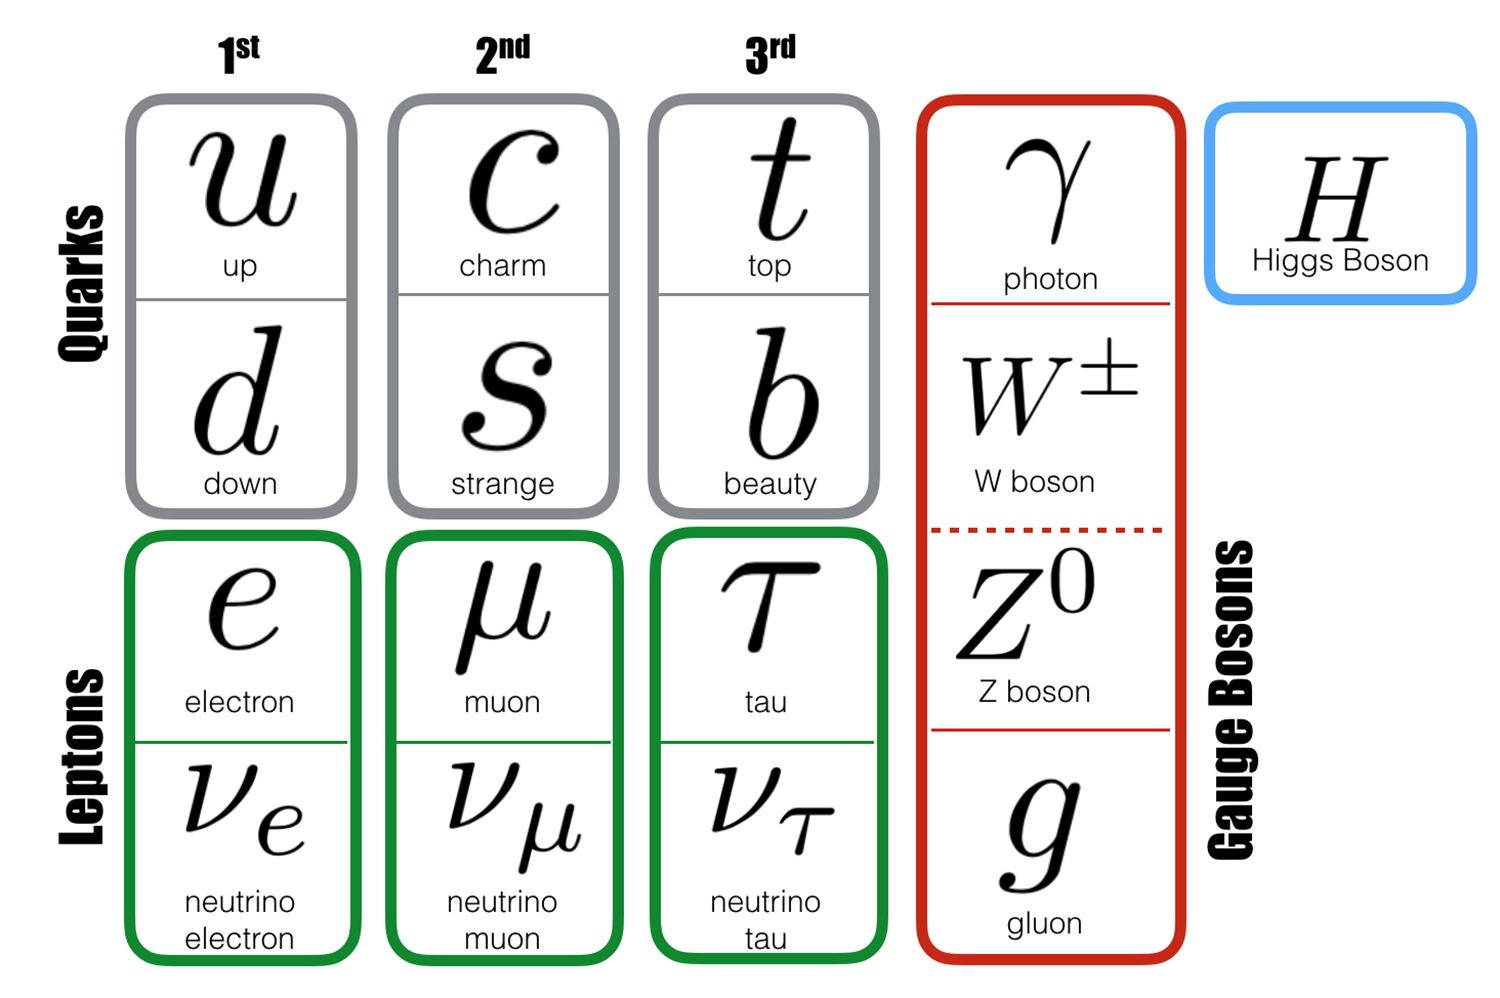
\includegraphics[width=0.80\linewidth]{figs/SM.png}
  \caption{Summary of elementary SM particles. The first three columns give
           the three generations of matter particles. Image taken
           from the Physics Institute at University of 
           Zurich~\cite{zurich_SM}.}
  \label{fig:SM}
\end{figure}

The theoretical framework underlying the SM is an example of a Quantum 
Field Theory (QFT). QFTs are consistent with both quantum mechanics and
relativity. Lattice gauge theories are a kind of QFT; therefore it is
important for the reader to know a little bit about them. There are a lot
of different resources one can use to learn about QFT; for example when I was a
grad student I used Peskin and Schroeder~\cite{peskin_introduction_1995}
and Srednicki~\cite{srednicki_quantum_2007}.
Nowadays there are also some very high quality lectures on YouTube,
for instance a series by Tong~\cite{tongQFT}, which I found had some other nice
introductory remarks. 
A timeline of particle discoveries can be found in
Ref.~\cite{wiki_particle_discoveries}. Another detailed historical overview
of the SM is given in Chapter 1 of Ref.~\cite{griffiths_introduction_2007}.

\section{An mnemonic history of the SM}

One could argue that the beginning of the SM history coincides with the
beginnings of modern particle physics. Since that depends on unifying
relativity, quantum mechanics, and field theory, one could arguably even take
Maxwell's equations as a starting point. 
There were also many interesting ideas that were not pursued or turned out
not to be correct yet still played some role in the history; I will not
discuss these. In some cases I may miss some discoveries that were also
important but less celebrated.

Given these ambiguities and the fact
that I am not at all a real historian, 
one might call what follows an ``approximate" history.
As I was writing this, I realized that I was trying to tell a story, i.e.
to write it in a way that one development would make sense or feel
motivated given a previous development. Usually that is a bit of an
oversimplification, but it helps me remember why certain discoveries were
significant, where some nomenclature comes from, and what it means. Hopefully it
also helps reveal how physicists think, how we are led to discoveries, and
ultimately why we believe our theories. So with these advantages in mind, I
rather decided to call it a ``mnemonic" history. 

Also while I was writing this, I learned a bunch of facts that I found
interesting but are probably a bit off-topic. Hence this mnemonic history is
densely packed with footnotes. For example I decided to start listing Nobel
prizes for some reason. By the time I realized doing this is tedious and doesn't
teach much, I somehow already felt pot-committed, so I ended up seeing this habit
through to the bitter end. 

\subsection{The fundamentals}

% pauli, jordan etc 1920s-30s how to quantize fields. 
% Failing to have theory with infinite num of dof,
% then tomonaga, schwinger, dyson, feynman. Can renormalize, QED discovered.
%   measurement of Lamb shift 1947. Bethe has explanation that gets refined
%   in QED, helps establish QFT.
% 1970s golden age: infinites understood through
% renormalization group wilson and kadanoff.

In 1897 J.J. Thomson did experiments with cathode rays\footnote{In a small
vacuum chamber with two electrodes, if a voltage is applied between them,
electrons will move between them. Televisions used to work by cathode ray tubes,
\index{cathode ray tube} where these electrons are deflected by magnetic fields
to make images on the screen.}
from which he concluded that electric charge must be carried by particles
with high charge-to-mass ratio, the electrons\footnote{He received the 1906
Nobel in physics for this work.} 
To explain why atoms are overall electrically neutral, Thomson guessed that
electrons are distributed in a sea of positive charge, which is the
well known {\it plum pudding model}.\index{plum pudding model} This was
disproved by Rutherford in his famous gold foil
experiment~\cite{rutherford_scattering_1911}, in which he discovered
the atomic nucleus. Shortly thereafter, he discovered the
proton~\cite{rutherford_collision_1919}.
Bohr proposed his model~\cite{bohr_constitution_1913}
of hydrogen, supposing it to be made of a proton and an electron, which agreed
well with experiment\footnote{He got the 1922 Nobel for his
contributions understanding atomic structure.}. Extending this theory to 
heavier elements by supposing
they are also made of only protons and neutrons however fails, since e.g. helium
is four times as heavy as hydrogen. This difficulty would not be sorted out
until the early 1930s, when Chadwick discovered~\cite{chadwick_possible_1932}
the neutron\footnote{1935 Nobel for him.}.


These early discoveries successfully explained many details of the atom; however
the fact that atomic nuclei are made of particles with only positive or zero
electric charge still required explanation.
Hence for some time, physicists
knew there must be some {\it strong force}\index{force!strong} that opposes
Coulomb repulsion and binds nucleons into nuclei.
Such particles held together by strong interactions are called
{\it hadrons}.\index{hadron} Nowadays we also use the terms {\it meson}
\index{meson} and {\it baryon}\index{baryon} to refer to hadrons made of
two quarks and three quarks, respectively\footnote{This naming scheme
comes from particle weights. At the time, known leptons were light, 
baryons were heavy, and mesons were somewhere in the middle. In retrospect it
would have been nicer to name them something like $n$-hadrons, but alas it would
take several decades for us to see that hadrons are made of quarks.}.


One of the earliest, important discoveries of the quantized natures of particle
properties is the celebrated Stern-Gerlach
experiment~\cite{gerlach_experimentelle_1922a,gerlach_magnetische_1922b,gerlach_experimentelle_1922c}. 
In this experiment, silver atoms
are deflected by an inhomogeneous magnetic field.
Besides having demonstrated that particles have intrinsic spin, it showed that
the spin is quantized and that measurements of spins along perpendicular axes
``reset" the spin state, and it provided the first measurement of the electron
magnetic moment.


Around this time, physicists were also beginning to see the particle nature of
light. In particular, Planck proposed~\cite{Planck:1901tja} 
that light may come in discrete packets of
energy in order to avoid the \index{ultraviolet catastrophe}ultraviolet 
catastrophe\footnote{1918 Nobel.}.
Einstein took this proposal seriously~\cite{Einstein:1905cc}, 
and used it to explain the photoelectric
effect\footnote{1922 Nobel for him. Also in 1905 he published his first
papers on special relativity, as well as a paper on Brownian motion.}. 
A careful study~\cite{millikan_direct_1916} of the photoelectric effect by 
Millikan showed that
Einstein's interpretation explained the photoelectric effect well\footnote{He
got the 1923 Nobel in part for this reason.}. Finally
Compton showed\footnote{He shared the 1927 Nobel for this.} 
that light scattered from a particle shifts by the Compton
wavelength\index{wavelength!Compton}
\begin{equation}
  \lambda_c=\frac{\hbar}{2mc},
\end{equation}
where $m$ is the target particle's mass, which one can derive by assuming light
is made of particles with zero rest mass~\cite{Compton:1923zz}.
Altogether these discoveries convinced physicists light behaves as a particle
at short enough length scales, which is the usual photon.\index{photon}


If light is to be quantized, it requires a theory that knows about both quantum
mechanics and special relativity, i.e. it needs QFT. 
The standard line of thinking can be cast in this way: One starts with
the Schr\"odinger 
equation~\cite{Schrodinger:1926gei,Schrodinger:1926vbi,Schrodinger:1926qnk,Schrodinger:1926xyk}
for a spinless, non-relativistic particle
of mass $m$ in the position basis,
\index{Schr\"odinger equation}
\begin{equation}
i\hbar\partial_t\psi=-\frac{\hbar^2}{2m}\nabla^2\psi.
\end{equation}
If we instead use a relativistic Hamiltonian and square the differential
operators on each side, we get the 
{\it Klein-Gordon equation}~\cite{Klein:1926tv,gordon_comptoneffekt_1926}
\index{Klein-Gordon equation}
\begin{equation}
-\hbar^2\partial_t^2\psi=\left(-\hbar^2c^2\nabla^2+m^2c^4\right)\psi.
\end{equation} 
While this is at least relativistically sensible, one can show that this
squaring of operators
leads to state normalization being time-dependent, i.e. probability is not
conserved. The situation was finally rescued by Dirac\footnote{Dirac
and Schr\"odinger shared the 1933 Nobel.}, who realized that
one could have a relativistically sensible equation that is first-order
in its operators by introducing some matrices and a spin component
to the wavefunction~\cite{Dirac:1928hu,Dirac:1928ej}. The result is the 
{\it Dirac equation}\index{Dirac equation}
\begin{equation}
i\hbar\slashed{\partial}\psi=mc\psi.
\end{equation}

The corresponding Hamiltonian for the Dirac equation is traceless, which
tells you that the energy eigenvalues cancel out, i.e. 
it suggests there are states of
negative energy. These negative energy states indicate that the theory
has no ground state. In order to prevent this infinite cascade into increasingly
negative energies, he speculated that these infinitely many states are already
occupied, which is referred to as \index{Dirac sea}the {\it Dirac sea}; 
the Pauli exclusion principle then prevents this infinite descent. 
If an electron in the sea were excited, it would leave behind a vacancy
that would manifest itself as a positively charged particle. This was the
prediction of the existence of the \index{positron}positron, which
was discovered\footnote{1936 Nobel.} in 1932 by Anderson~\cite{Anderson:1933mb}.
Later St\"uckelberg~\cite{Stueckelberg:1941rg} and
Feynman~\cite{feynman_theory_1949} would introduce the modern interpretation
of the positron: rather than being a hole left in the Dirac sea,
the previously negative energy states are to be understood as the
positive energy states of a different particle.


One of the last kinds of fermions needed to complete our particle collection
are the neutrinos. Before 1930, there was a problem with $\beta$-decay
\index{decay!beta} 
which is any decay emitting an $e^+$ or $e^-$ from
an atomic nucleus: Energy was not conserved. In particular if one assumes
a general $\beta$-decay process functions like
\begin{equation}
  A\to B+e^-,
\end{equation}
one can use conservation of four-momentum to find the electron energy.
The measured energy was found to fluctuate and be smaller than what four-momentum
conservation delivers. Pauli
suggested\footnote{Rather than being documented in a publication, this seems to
come from a letter written by Pauli addressed to a conference in T\"ubingen.
It opens, ``Liebe Radioaktive Damen und Herren".} that this missing energy
lies with an as-yet-undetected, weakly interacting particle, the
electron neutrino. The electron neutrino would not be 
discovered\footnote{1995 Nobel.}\index{neutrino!electron}
until the mid 1950s by Cowan and Reines~\cite{Cowan:1956rrn}.

\subsection{Weak and strong forces}

\index{interaction!weak}
In the early 1930s, Fermi published\footnote{Apparently he originally attempted
to publish it in {\it Nature}, but they rejected it because
it because ``it contained speculations too remote from reality to be of interest
to the reader".} his theory of the 
\index{decay!beta}$\beta$-decay~\cite{fermi_tentativo_1934}
\begin{equation}
  n\to\text{p}+e^-+\bar{\nu}_e.
\end{equation}
He introduced an effective 4-point interaction directly linking the four
particles in the above process.
Shortly thereafter, Yukawa~\cite{yukawa_interaction_1935} put forward that this
interaction should include another field with corresponding quantum that
mediates this interaction\footnote{Nowadays we designate as
{\it Yukawa interaction} any interaction between
Dirac fields and scalar fields of the form\index{interaction!Yukawa}
$g\bar{\psi}\phi\psi$ or $g\bar{\psi}i\gamma_5\phi\psi$.}, 
sort of like how the photon mediates the
electromagnetic interaction. Another salient point of this paper is
the introduction of the {\it Yukawa potential}\index{potential!Yukawa}
giving the potential of a gauge boson of mass $m$:
\begin{equation}
  V(r)=-g^2\frac{e^{-\alpha m r}}{r}.
\end{equation}
Here $g$ is the gauge coupling and $r$ is the interaction range. One sees that
massless gauge bosons have a Coulomb-like potential, while massive ones
are suppressed exponentially\footnote{One can also show that the Fourier
transform of this potential is the propagator, which we will discuss later.},
which gives an explanation why the weak force has a short interaction range. 
Besides already hinting massive weak bosons, this paper is considered to be
one of the first theories of the strong force; from this perspective the
proton and neutron exchange massive mesons, which therefore have a limited
interaction range\footnote{1949 Nobel.}.

\begin{figure}
  \centering
  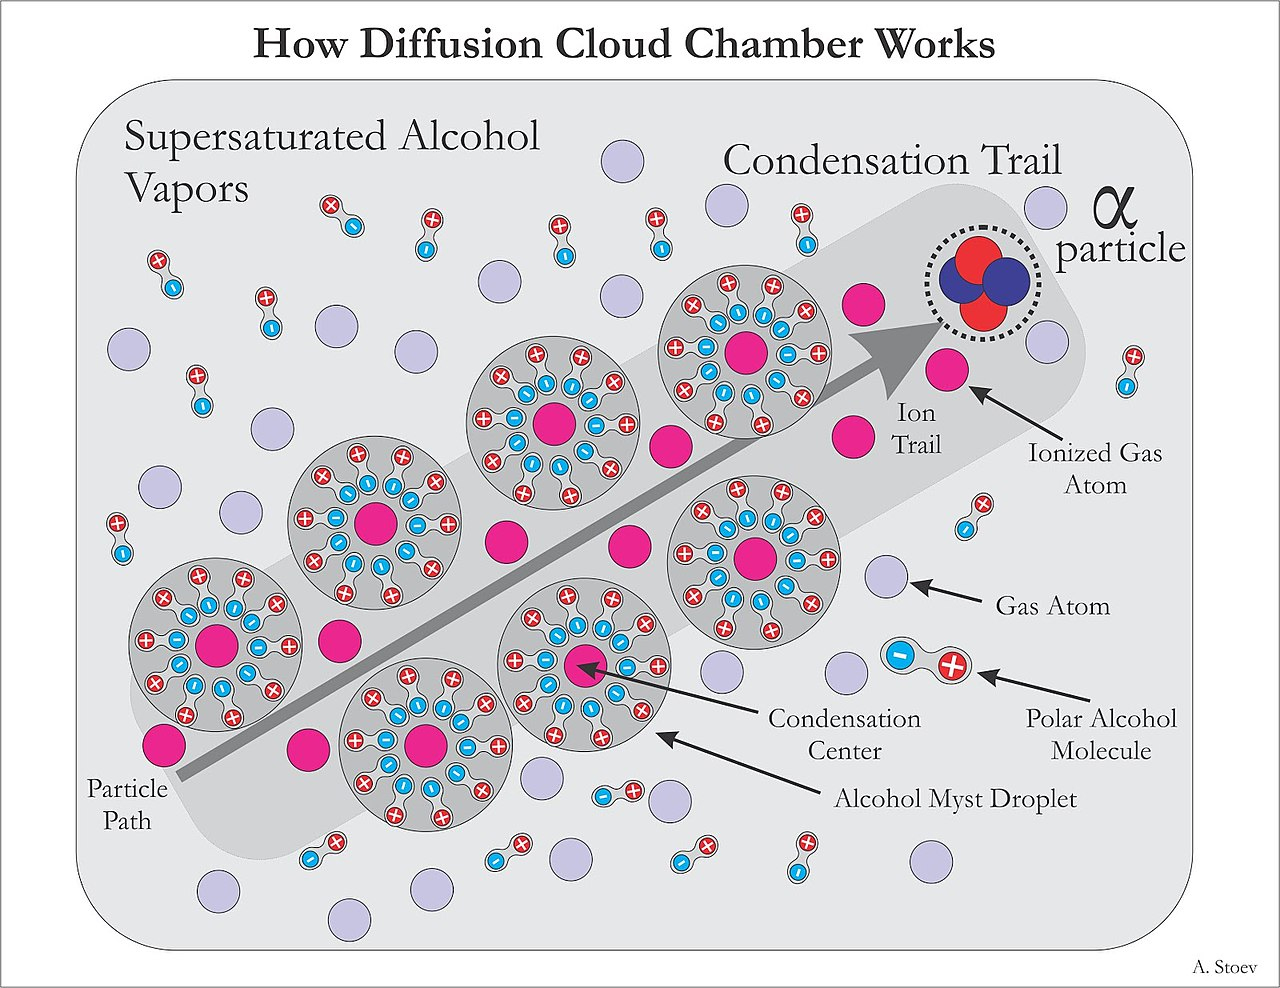
\includegraphics[width=\linewidth]{figs/Diffusion_Cloud_chamber_explained.jpg}
  \caption{Cloud chambers consist of a sealed environment with some vapor
           of e.g. alcohol. As a charged particle moves through the vapor, it knocks
           electrons off the gas; the resulting ions attract the polar molecules,
           which leaves a visible trail for a short time. To identify particles,
           you can see e.g. if they were deflected. C. T. R. Wilson is generally 
           credited as the inventor of cloud chambers, and he shared the 1927 Nobel
           in physics for it. They were extremely popular to use in experiment
           for finding particles until the later invention of the bubble chamber.
           Image taken from Wikipedia~\cite{wiki_cloud}.}
  \label{fig:cloud}
\end{figure}

An early experimental search of cosmic ray\footnote{A {\it cosmic ray} is a high
energy proton or atomic nucleus that originates somewhere from space. They were
discovered in the early 1910s by Hess, which got him the 1936 Nobel.}
\index{cosmic ray} measurements using
cloud\index{cloud chamber} chambers (see \figref{fig:cloud}) 
found the muon~\cite{neddermeyer_note_1937}, which was originally 
mistaken\footnote{Indeed the muon and pion masses are pretty close to each
other, sitting at about 106~MeV and 140~MeV, respectively.}
as the meson that Yukawa suggested. An experiment in the late 1940s showed that
the muon does not interact very strongly with atomic
nuclei~\cite{conversi_disintegration_1947}, which rules it out as the strong
force mediator. Thankfully for Yukawa the pion was
discovered~\cite{lattes_processes_1947} in 1947\footnote{And got Powell
the 1950 Nobel for it. It is actually a bit puzzling that he is the only
recipient of this prize, most obviously because only three other scientists were
on his team. Furthermore this prize credits him for his ``development of
photographic method for studying nuclear processes", even though this method was
pioneered by other physicists such as Blau and Wambacher.}.


\index{interaction!strong}
In the late 1940s and early 1950s, the {\it kaon} ($K$)~\cite{rochester_evidence_1947}
\index{meson!K} and {\it lambda} ($\Lambda$)~\cite{hopper_evidence_1950}
\index{baryon!lambda} hadrons were discovered. A kaon
consists of light quark and a strange, while a lambda baryon binds two light
quarks with one from a higher generation. {\it Strangeness}\footnote{We now 
\index{strangeness}
identify strangeness $S$ as
$$
  S\equiv\#\,\text{anti-strange quarks}-\#\,\text{strange quarks}.
$$}
was originally proposed as a conserved quantity to explain the relatively long
lifetimes of these particles~\cite{pais_remarks_1952,gell-mann_isotopic_1953,
pais_baryon-meson-photon_1953,tadao_charge_1953}.
Ne'eman~\cite{neeman_derivation_1961},
Gell-Mann~\cite{gell-mann_symmetries_1962}, and
Zweig~\cite{zweig_su3_1964} proposed\footnote{Gell-Mann would receive the 1969
Nobel for his contributions to understanding elementary particle
classification.} that these hadrons could be classified
according to the irreducible representations of $\SU(3)$, a viewpoint which
Gell-Mann called the \index{eightfold way}{\it eightfold way}\footnote{This
name is inspired by the eightfold path of Buddhism.}, examples of which are
illustrated graphically in \figref{fig:eightfold}. Gell-Mann
referred to the fundamental units as {\it quarks}\footnote{Gell-Mann borrows
this name from an excerpt of James Joyce's {\it Finnegan's Wake} that begins
``Three quarks for Muster Mark".
Gell-Mann was a bit of a fanciful guy I guess.}.
At first it was not clear that this quark viewpoint was more than a
purely mathematical construction, however deep inelastic
scattering\index{scattering!deep inelastic}
experiments at the Stanford Linear Accelerator (SLAC) showed that
protons are made of smaller particles, and are therefore not
elementary~\cite{bloom_high-energy_1969,breidenbach_observed_1969}.
This alone did not convince the community that quarks were 
real\footnote{For a while it was fashionable to refer to rather refer to
nucleon constituents as {\it partons}\index{parton}, a term coined
by Feynman.}, but
subsequent discoveries would solidify the quark model.

\begin{figure}[t]
  \centering
  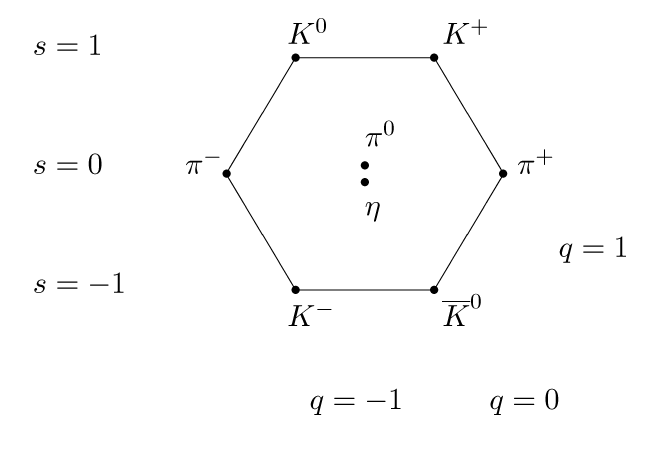
\includegraphics[width=0.48\linewidth]{figs/Meson_octet.png}
  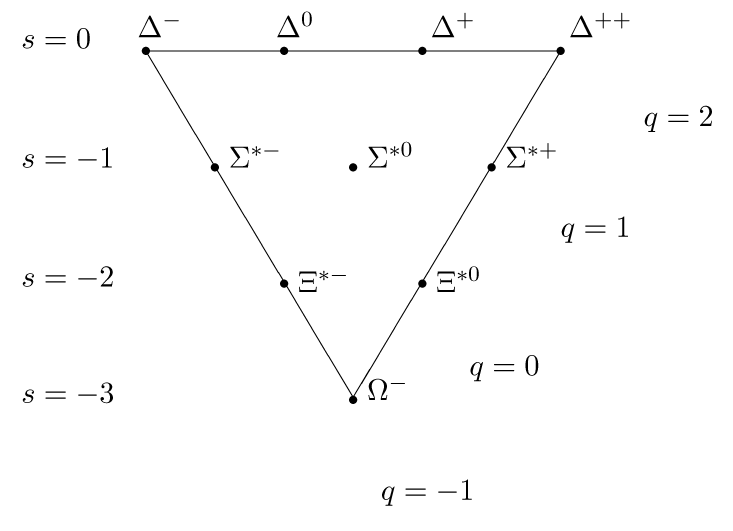
\includegraphics[width=0.48\linewidth]{figs/Baryon_decuplet.png}
  \caption{{\it Left}: Spin-0 pseudo-scalar meson octet. {\it Right}:
           Spin-3/2 baryon decuplet. The $s$ represents strangeness,
           with all particles in the same horizontal row having the
           same strangeness. Electric charge is represented by $q$,
           with all particles along the diagonal having the same
           electric charge. Images taken from
           Wikipedia~\cite{wiki_eightfold}.}
  \label{fig:eightfold}
\end{figure}

From here it was shown possible to formulate a QFT for the strong interaction
based on $\SU(3)$~\cite{fritzsch_advantages_1973}, which we
call quantum chromodynamics (QCD).\index{quantum chromodynamics}
The mediators are called
{\it gluons}\index{gluon} with the adjoint representation delivering
eight possible color combinations.
Gross, Wilczek~\cite{gross_d.j._ultraviolet_1973} and
Politzer~\cite{politzer_reliable_1973} demonstrated
{\it asymptotic freedom}\footnote{They got the 2004 Nobel for this.}
\index{asymptotic freedom} in this QFT, i.e. they showed that the
strong coupling decreases with increasing interaction strength, which is
consistent with the fact that one does not observe free quarks\footnote{At
least not at typical temperatures and densities.}.
This theoretical observation is buttressed by strong coupling
expansions in the lattice formulation, introduced by 
Wilson~\cite{wilson_confinement_1974}, which show that the potential
energy between two infinitely heavy quarks grows linearly with
increasing separation
(see \secref{sec:hqfe}).
%creutz_monte_1980
%wilson_RG 1 and 2

We round out this section with a short timeline of discoveries of the
remaining QCD particles. In 1974 the discovery of the
$J/\Psi$-meson\index{psion} or {\it psion}\footnote{The $J/\Psi$ consists
of a $\bar{c}c$ pair. This is also sometimes called {\it charmonium}.
\index{charmonium}} at both Brookhaven National Lab (BNL) and
SLAC~\cite{augustin_discovery_1974,aubert_experimental_1974} demonstrated
the existence of the charm quark\footnote{Richter and Ting got the 1974
Nobel prize in physics for this.}, adding further evidence to
the validity of the quark model. The $J/\Psi$ discovery marks the beginning of a
period of rapid discoveries in particle physics sometimes referred to as the
``November Revolution".\index{November Revolution} The existence of the bottom
quark was demonstrated in 1977 at Fermilab~\cite{herb_observation_1977} when the
$Y$-meson\footnote{A $Y$-meson\index{meson!Y} is a $\bar{b}b$ bound state. This is
sometimes called \index{bottomonium}{\it bottomonium}.} was discovered.
In 1979 we found experimental evidence for the
gluon via indirect observations~\cite{barber_discovery_1979} at the
Deutsches Elektronen-Synchrotron (DESY). In part because it is the
heaviest quark, the top quark would not be discovered until
1995~\cite{abachi_observation_1995,abe_observation_1995}
at Fermilab.


\subsection{Unification}


In the mid 1950s, Lee and Yang~\cite{lee_question_1956} suggested possible
experimental tests to search for parity violation in weak interaction 
processes\footnote{Lee and Yang won the 1957 Nobel prize for this.}.
Shortly thereafter, Wu et al.~\cite{wu_experimental_1957} demonstrated parity
violation in the $\beta$-decay of \ce{^{60}Co},
a result which was verified by Garwin et al.~\cite{garwin_observations_1957}. 
The theory of the weak interaction was extended by Gell-Mann and
Feynman~\cite{feynman_theory_1958} to accommodate parity violation by
introducing vector-axial currents.
That $\beta$-decay proceeds through vector-axial currents was
experimentally verified shortly thereafter~\cite{goldhaber_helicity_1958}.


The unification of the weak and electromagnetic forces began already with
Glashow in 1961~\cite{glashow_partial-symmetries_1961}, where
he puts forward the $\SU(2)\times \U(1)$ symmetry group. 
Still, this theory was not known to be renormalizable.
Also the weak interaction is short range, but this suggests that the mediating boson 
should be massive according to Yukawa. On the other hand, 
massive gauge bosons superficially spoil gauge invariance.


In superconductivity, Ginzburg-Landau theory~\cite{ginzburg_theory_1950}
gives solutions with effective mass. Nambu applied\footnote{2008 Nobel prize.} 
this to particle
physics~\cite{nambu_axial_1960,nambu_dynamical_1961,nambu_dynamical_1961-1},
but this implied the existence of Goldstone modes that are not observed.
Higgs~\cite{higgs_broken_1964} and Brout and Englert~\cite{englert_broken_1964}
noticed\footnote{Higgs and Englert received the 2013 Nobel for this.} 
that by strategically choosing 
the gauge, one can simultaneously
eliminate the Goldstone modes, add a mass term to gauge bosons, and a scalar
boson, the Higgs boson.\index{boson!Higgs}
We will discuss spontaneous symmetry breaking and Goldstone's theorem
\index{spontaneous symmetry breaking} in \secref{sec:ssb}. The Higgs
mechanism is discussed in detail in \apref{ap:spec_higgs}.


The original Higgs-Brout-Englert mechanism was demonstrated only for massive
QED; Kibble extended this idea to non-abelian
groups~\cite{kibble_symmetry_1967}. Weinberg~\cite{weinberg_model_1967}
and Salam~\cite{salam_weak_1968} applied Kibble's results to Glashow's
$\SU(2)\times\U(1)$ idea\footnote{And shared the 1979 Nobel for it.}. 
They demonstrated that one can generate masses
for weak gauge bosons along with electrons and muons, while still leaving
neutrinos massless. This approach also predicted neutral weak currents,
which were discovered shortly thereafter by the Gargamelle
experiment~\cite{hasert_observation_1974}. The $W$ and $Z$ bosons would
be discovered at the European Organization for Nuclear Research (CERN)
in the early 1980s~\cite{aubert_ratio_1983,arnison_experimental_1983}.


In 1963, Cabibbo introduced the {\it Cabibbo angle}\index{Cabibbo angle} allowing
for quark mixing in weak interactions~\cite{cabibbo_unitary_1963} to
explain the lifetimes of heavier hadrons. The suppression of flavor changing
neutral currents was explained in the early 1970s through the GIM\index{GIM mechanism}
mechanism~\cite{glashow_weak_1970}, but in order for this mechanism to work,
one needed full doublets of quarks and leptons.
Then Kobayashi and Maskawa predicted the existence of a third
generation~\cite{kobayashi_cp_1973}, since three quark generations are the
minimal amount needed to allow CP violation in the quark sector\footnote{They
shared the 2008 Nobel along with Nambu.}. The full quark mixing matrix
is known as the CKM matrix.\index{CKM matrix} Neutrino mixing is also handled
through a mixing matrix, the so-called PMNS matrix.\index{PMNS matrix} 
We discuss neutrino mixing in detail
in \apref{ap:spec_neutrino}.


In the early 1970s, t'Hooft and Veltman
showed\footnote{1999 Nobel prize for them.} these theories are
renormalizable~\cite{t_hooft_regularization_1972}. Together the Higgs mechanism
and renormalizability of the SM allow one to consistently generate gauge boson
masses while ensuring its applicability at all energy scales.
Furthermore CERN's 2012 discovery of the Higgs 
boson~\cite{aad_observation_2012,chatrchyan_observation_2012} shows that Higgs mechanism
corresponds to reality, rather than being just a mathematical trick to 
consistently approach massive elementary particles.



\section{Introductory remarks about QFT} 

Here I just want to list some things that seem to be true about the universe,
and therefore our underlying theory should reflect these things. For example:
\begin{enumerate}
  \item Causal influences seem to be {\it local}, i.e. there is no
        action-at-a-distance.
  \item Elementary particles are completely and perfectly indistinguishable.
\end{enumerate}
One way to make sense of these two points is to assume the existence of 
{\it fields},\index{field} math objects whose pre-image is all space-time.
That the field value depends on its space-time coordinate allows it to be local,
and all elementary particles are viewed as excitations of the field. Since all
particles are excitations of the same object, it is therefore unsurprising that
they would be indistinguishable.

Related to point (1) above, and as already mentioned in the introduction, we
would like our theories to have this property:
\begin{enumerate}
  \setcounter{enumi}{2}
  \item QFT should be consistent with special relativity.
\end{enumerate}
Demand (3) leads in part to the Klein-Gordon and Dirac equations, and from these
we will find that particle number is not conserved.
A fundamental QFT length scale can be heuristically derived from this statement 
as follows: Consider an elementary particle in a box of length $L$. By the 
uncertainty principle, we have
\begin{equation}
  \Delta p\gtrsim \hbar/2L,
\end{equation}
which means according to relativity,
\begin{equation}
  \Delta E\gtrsim \hbar c/2L.
\end{equation}
If the energy uncertainty is large enough, i.e. large enough to support a
particle-antiparticle pair, we conclude
\begin{equation}
  \Delta E\approx 2mc^2 \gtrsim\hbar c/2L.
\end{equation}
Appearing in this equation is the Compton wavelength\footnote{I guess if
one uses $\hbar$ instead of $h$ this is rather the {\it reduced} Compton
wavelength. But I somehow always work using $\hbar$ instead of $h$, so I opted
to abuse this convention a little.}\index{wavelength!Compton}
$\lambda_c=\hbar/mc$. This delivers an interpretation for the Compton wavelength:
\begin{equation}
  L \gtrsim \lambda_c/4
\end{equation}
is a distance threshold\footnote{I have also seen $\lambda_c/2$ as the threshold,
which comes when you think the energy uncertainty only has to be large enough to
support a single particle. But in QFT particles are always created from the
vacuum in particle-antiparticle pairs due to conservation laws.} below which 
you have to worry about QFT. Below this scale, you are likely to detect
particle-antiparticle pairs of the species you are examining, which you cannot
distinguish, and it becomes difficult to speak a unique particle at all. In that
sense the Compton wavelength gives a characteristic length scale for a
particle. One can compare this with the particle's de Broglie wavelength
\index{wavelength!de Broglie}$\lambda_v=\hbar/mv$, where it behaves in a well-defined way as a wave.


\section{The principle of stationary action}


This section follows a fairly well known and delightful lecture by Feynman
\cite{caltech}.

\index{limit!classical}\index{non-relativistic limit}
\section{The non-relativistic and classical limits}

In this section I briefly give some intuition for how mundane Newtonian
physics can be recovered from the more esoteric relativistic and quantum
theories. Namely \index{limit!non-relativistic} I want to focus on 
the following two phrases:
\begin{enumerate}
  \item The non-relativistic limit is $c\to\infty$.
  \item The classical limit is $\hbar\to0$.
\end{enumerate}
I don't think I have the understanding to prove anything, but at least I
can provide some ideas and examples that can make you believe these
two statements.

The non-relativistic limit is, I think, the easier to understand. When we
learn about relativity, the speed of light $c$ is taken as a ``cosmic speed
limit"; correspondingly, sending $c\to\infty$ lifts the speed limit, and
so perhaps it's not surprising that Galilean physics is recovered.
More explicitly, we can see what happens to the Lorentz factor $\gamma$ and
Einstein velocity addition formula under these limits. For the former
we find
\begin{equation}
  \lim_{c\to\infty}\gamma
  =\lim_{c\to\infty}\frac{1}{\sqrt{1-v^2/c^2}}=1,
\end{equation}
i.e. there is no longer any time dilation or length contraction.
Meanwhile when $c\gg v$, we find for the velocity addition formula 
\begin{equation}
  v_1\oplus v_2
  =\frac{v_1/c + v_2/c}{1+v_1v_2/c^2}
  \approx \frac{v_1}{c} + \frac{v_2}{c}, 
\end{equation}
i.e. it reduces to Galilean velocity addition.

For the classical limit, one can look at specific, simple examples, such as
the quantum harmonic oscillator. In QM, the energy levels of this system
are given by
\begin{equation}
  E_n=\hbar\omega\left(n+\frac{1}{2}\right).
\end{equation}
In the $\hbar\to0$ limit, one therefore sees that the differences in energy
become continuous rather than discrete. More generally one can look at
the Heisenberg uncertainty relation,
\begin{equation}
  \Delta p\Delta x\geq \frac{\hbar}{2},
\end{equation}
and when $\hbar=0$, you are once again allowed to know position and
momentum simultaneously.

% TODO: path integral classical limit

%\section{The path integral}

%\section{Discrete symmetries}\label{sec:discreteSymm}

\section{Vacuum polarization}\label{sec:VP}\index{vacuum polarization}

For this section we closely follow Ref.~\cite{maiani_hadron_2016}, 
which I found to be quite
a nice introduction to vacuum polarization.

The simplest case of {\it vacuum polarization} (VP) is a one-loop effect in
$e^+e^-$ scattering in QED. If the virtual photon has enough energy,
an $e^+e^-$ pair can be emitted and reabsorbed, and this
pair will effectively screen\footnote{The name can be remembered in analogy to
the application of an external magnetic field on a dielectric material.
In this case the polarized molecules in the material will also screen
the external field inside the material.} the electromagnetic field, reducing the force
carried by the photon.

Any possible charged particle-antiparticle pair must be considered,
for instance $\mu^+\mu^-$ and $\tau^+\tau^-$. Their effects are small compared
to $e^+e^-$ due to their comparatively large masses, and are hence
only noticeable for large\index{virtuality} {\it virtuality}, or $q^2$,
of the exchanged photon. 
Contributions to VP coming from strongly interacting particles
is referred to as\index{vacuum polarization!hadronic} 
{\it hadronic vacuum polarization}.
Their effect can be computed perturbatively at large $q^2$,
but at small $q^2$ this of course fails.

The first experimental indication of HVP was found at LAL-Orsay~\cite{},
which measured the cross section for $e^+e^-\to\mu^+\mu^-$.
There a characteristic interference pattern was found for
the $\phi(1020)$ resonance, in concordance with the
$\phi$ HVP contribution. CERN had a series of experiments
starting in 1958~\cite{}, culminating
in the measurement of the\index{anomalous magnetic moment!muon}
{\it muon anomalous magnetic moment},
\begin{equation}
  a_\mu=\frac{g_\mu-2}{2},
\end{equation}
where $g_\mu$ is the muon gyromagnetic ratio,
which agreed at the time with the SM~\cite{}.
We will discuss this in more detail in \secref{sec:anomMuon}

Since then,
higher precision was achieved at Brookhaven~\cite{},
exhibiting XX tension against the SM.
This program of increased experimental precision
is being continued at Fermilab and J-PARC;
the state-of-the-art determination from 
Fermilab~\cite{}
places experimental searches at XX tension
against so-called dispersive methods,
which we will discuss shortly.
At the same time, the BMW collaboration achieved
the (at that time) highest precision lattice determination
of (HVP?), results that XX with the SM~\cite{};
since then many other lattice determinations 
by the XX group, YY group,... ~\cite{} have
confirmed their result.
(Also explain any limitations?)

It is abundantly clear that this situation is in dire need
of clarification. (Especially with respect to the above
limitations, what is the new thing your calculation provides?)

% section 6 of that nice review
\subsection{Muon anomalous magnetic moment}\label{sec:anomMuon}

\begin{equation}
  \vec{M}=g_\mu\frac{e}{2m_\mu}\vec{S}
\end{equation}
\begin{equation}
  a_\mu^{\rm SM}
\end{equation}



\section{Isospin and hypercharge}\label{sec:isohyper}
\index{hypercharge}\index{isospin}

We follow Chapter~9 of 
Thomson~\cite{thomson_modern_2013}. 
In quantum mechanics you learn that spin is a quantum number of
charged particles. For example the electron is a spin-1/2 particle. The
$z$-component $S_3$ of the spin operator $S$ commutes with the Hamiltonian, and
you learn that the eigenvectors of $S_3$ are the +1/2 and -1/2 states. You also
learn that the components of $S$ are related to the Pauli matrices by
\begin{equation}
  S_i=\frac{\hbar}{2}\sigma_i.
\end{equation}

Early on in nuclear physics, scientists noticed that the proton and neutron had
about the same mass, and that the nuclear force between two nucleons (i.e.
protons or neutrons) was approximately charge independent. Therefore Heisenberg
suggested that protons and neutrons were two states of a single particle (the
nucleon) just as there are spin-up and spin-down states of a spin-1/2
particle.
The quantum number corresponding to this property is called {\it isospin}.
Using this idea, the proton and neutron form an isospin doublet with total
isospin $I=1/2$ and $z$-component $I_3=\pm1/2$. Thus the Pauli matrices also
give a suitable representation of the isospin operator, and we write
\begin{equation}
  I^2=\sum\limits_{i=1}^3 I_i^2, \qquad I_i=\frac{1}{2}\sigma_i.
\end{equation}
I know this is sloppy, but I want to leave it to the reader to determine from
context whether $I$ represents the operator or the eigenvalue. 

The concept of isospin can be extended in the same way to quarks. 
In the simplest case we have $N_f=2$ and consider the lightest quarks
$u$ and $d$. The $\SU(2)$ isospin symmetry is only approximate because 
the $u$ and $d$ quarks have slightly different masses. The isospin 
doublet then has a $u$ component and a $d$ component. Generally with
$N_f$ flavors of fermion with degenerate masses, the symmetry group is 
$\SU(N_f)$ and we
form $N_f$-component multiplets in flavor space, one component per flavor.

Let's introduce the $s$ quark, assuming it has the same mass as the
$u$ and $d$ quarks, and do the $N_f=3$ case.
Using the Pauli matrices and the fact that $\SU(3)$ has 8 generators, you can
figure out what the Gell-Mann matrices are. We will say that $u$, $d$, and $s$
are eigenvectors of isospin and write
\begin{equation}
  u=\colvec{3}{1}{0}{0}, \qquad
  d=\colvec{3}{0}{1}{0}, \qquad
  s=\colvec{3}{0}{0}{1}.
\end{equation}
Then $u$ and $d$ span a 2D subspace of flavor space, so from the earlier
discussion we should know that the generators of $\SU(2)$ are contained in the
generators of $\SU(3)$. Hence
\begin{equation}
  \lambda_1=\left(\begin{array}{ccc}
            0 & 1 &  \\
            1 & 0 &  \\
              &   & 0
            \end{array}\right), \qquad
  \lambda_2=\left(\begin{array}{ccc}
            0 & -i &  \\
            i & 0  &  \\
              &    & 0
            \end{array}\right), \qquad
  \lambda_3=\left(\begin{array}{ccc}
            1 & 0  &  \\
            0 & -1 &  \\
              &    & 0
            \end{array}\right).
\end{equation}
But there's nothing special about $u$ and $d$; $u$ and $s$ will similarly form
a subspace, and so will $d$ and $s$. In both cases, we will use the Pauli
matrices as generators. We can similarly write
\begin{equation}
  \lambda_4=\left(\begin{array}{ccc}
            0 &   & 1\\
              & 0 &  \\
            1 &   & 0
            \end{array}\right), \qquad
  \lambda_5=\left(\begin{array}{ccc}
            0 &    & -i \\
              & 0  &    \\
            i &    & 0
            \end{array}\right), \qquad
  \lambda_X=\left(\begin{array}{ccc}
            1 &    & 0 \\
              & 0  &   \\
            0 &    & -1
            \end{array}\right),
\end{equation}
\begin{equation}
  \lambda_6=\left(\begin{array}{ccc}
            0 &   &  \\
              & 0 & 1\\
              & 1 & 0
            \end{array}\right), \qquad
  \lambda_7=\left(\begin{array}{ccc}
            0 &    &   \\
              & 0  & -i\\
              & i  & 0
            \end{array}\right), \qquad
  \lambda_Y=\left(\begin{array}{ccc}
           0  &    &  \\
              & 1  & 0\\
              & 0  & -1 
            \end{array}\right).
\end{equation}
Finally note the fact that there are only 8 linearly independent generators, so
two of these matrices should be linearly dependent. Since the
$u\leftrightarrow d$ isospin symmetry is the closest to being exact, we choose
the last generator to be a linear combination of $\lambda_X$ and $\lambda_Y$
that treats the $u$ and $d$ quarks symmetrically. Thus
\begin{equation}
  \lambda_8=\frac{1}{\sqrt{3}}\lambda_X+\frac{1}{\sqrt{3}}\lambda_Y
           =\frac{1}{\sqrt{3}}\left(\begin{array}{ccc}
            1 &   &   \\
              & 1 &   \\
              &   & -2
            \end{array}\right).
\end{equation}
The new isospin and total isospin operators are
\begin{equation}
  I^2=\frac{1}{4}\sum\limits_{i=1}^8 I_i^2, \qquad I_i=\frac{1}{2}\lambda_i.
\end{equation}

In the case of $\SU(2)$, the operators $I_i$ do not commute, and therefore are
not simultaneously diagonalizable. For $\SU(3)$ in the Gell-Mann basis,
$I_3$ and $I_8$ are both diagonal, so they correspond to compatible
observables. The observable $I_3$ is itself sometimes referred to
as isospin or weak isospin. The observable we associate with $I_8$ is rescaled as
\begin{equation}
  Y=\frac{1}{\sqrt{3}}\lambda_8,
\end{equation}
and $Y$ is called the {\it hypercharge}.\index{hypercharge} 
We can quickly obtain the isopins and hypercharges of
our lightest quarks: 
\begin{equation}\begin{aligned}
\hat{I_3}\,u =\frac{1}{2}u ~~~ &\text{and}~~~\hat{Y}u=\frac{1}{3}u,\\
\hat{I_3}\,d =-\frac{1}{2}d ~~~ &\text{and}~~~\hat{Y}d=\frac{1}{3}d,\\
\hat{I_3}\,s = 0           ~~~ &\text{and}~~~\hat{Y}s=-\frac{2}{3}s.
\end{aligned}\end{equation}
One can summarize this pattern of conserved charges in the following formula:
\begin{theorem}{Gell-Mann-Nishijima Formula}{}
\index{Gell-Mann-Nishijima formula}
  The electric charge $Q$ of a particle is related to its isospin and
  hypercharge by
  \begin{equation*}
    Q=I_3+\frac{1}{2}Y
  \end{equation*}
\end{theorem}


\section{Spontaneous symmetry breaking}\label{sec:ssb}
\index{spontaneous symmetry breaking}
We follow Section~11.1 of Peskin and 
Schroeder~\cite{peskin_introduction_1995}.
Let $\phi(x)$ denote a vector (in the mathematical sense) of $N$ real,
scalar fields $\phi^i(x)$. Then the Lagrangian
\begin{equation}
  \Lagr=\frac{1}{2}\left(\partial_\mu\phi\right)^2
        +\frac{1}{2}\mu^2\phi^2-\frac{\lambda}{4}\phi^4
       \equiv\frac{1}{2}\left(\partial_\mu\phi\right)^2
        +V(\phi)
\end{equation}
is invariant under the orthogonal group\footnote{Recall orthogonal 
transformations\index{group!orthogonal} $R$ are the ones with 
$R^TR=\id$.} O$(N)$. This is the Lagrangian of the\index{sigma model}
{\it linear sigma model}. Note that is is a generalization of $\phi^4$ theory,
but we have replaced the positive mass parameter $m^2$ with a
negative parameter $-\mu^2$ and rescaled $\lambda$ to eliminate a factor of 6.
Classically, the potential is minimized when $\phi$ lies
on an $N$-dimensional sphere of radius $\sqrt{\mu^2/\lambda}$, i.e. 
it is minimized for vectors $\phi_\text{min}$ satisfying
\begin{equation}
  \phi_\text{min}^2=\frac{\mu^2}{\lambda}.
\end{equation}
To interpret the theory, we first choose coordinates so that 
$\phi_\text{min}$ lies
entirely along the $N$ direction
\begin{equation}\label{eq:phidir}
  \phi_\text{min}=(0,0,...,0,v),
\end{equation}
where $v=\sqrt{\mu^2/\lambda}$ is the {\it vacuum expectation value} or VEV.
Then, we define a set of shifted fields $\pi_k$ and $\sigma$ relative
to this point by writing
\begin{equation}\label{eq:phishift}
  \phi(x)=\left(\pi_1(x),\pi_2(x),...,\pi_{N-1}(x),v+\sigma(x)\right)
\end{equation}
Written in terms of $\pi$, the $N-1$ dimensional vector with components
$\pi_k$, and $\sigma$, the new Lagrangian becomes
\begin{equation}\label{eq:brokenlagr}
  \Lagr=\frac{1}{2}\left(\partial_\mu\pi\right)^2
        +\frac{1}{2}\left(\partial_\mu\sigma\right)^2
        -\frac{1}{2}\left(2\mu^2\right)\sigma^2-\sqrt{\lambda}\mu\sigma^3
        -\sqrt\mu\pi^2\sigma
        -\frac{\lambda}{4}\sigma^2
        -\frac{\lambda}{2}\pi^2\sigma^2
        -\frac{\lambda}{4}\pi^4,
\end{equation}
where we have removed constant terms, because they do not change the
physics. Equation~\eqref{eq:brokenlagr} is the Lagrangian of $N-1$
massless, dynamic fields $\pi_k$ and a dynamic field $\sigma$ with mass
$\sqrt{2}\mu$. Written in this form, the original $\text{O}(N)$ symmetry
is now obscured. There is a remaining $\text{O}(N-1)$ symmetry
rotating the $\pi_k$ among themselves. This is an example of
{\it spontaneous symmetry breaking} (SSB), and we say something like
``the original $\text{O}(N)$ symmetry spontaneously breaks to
the subgroup $\text{O}(N-1)$." 

\begin{figure}[t]
\centering
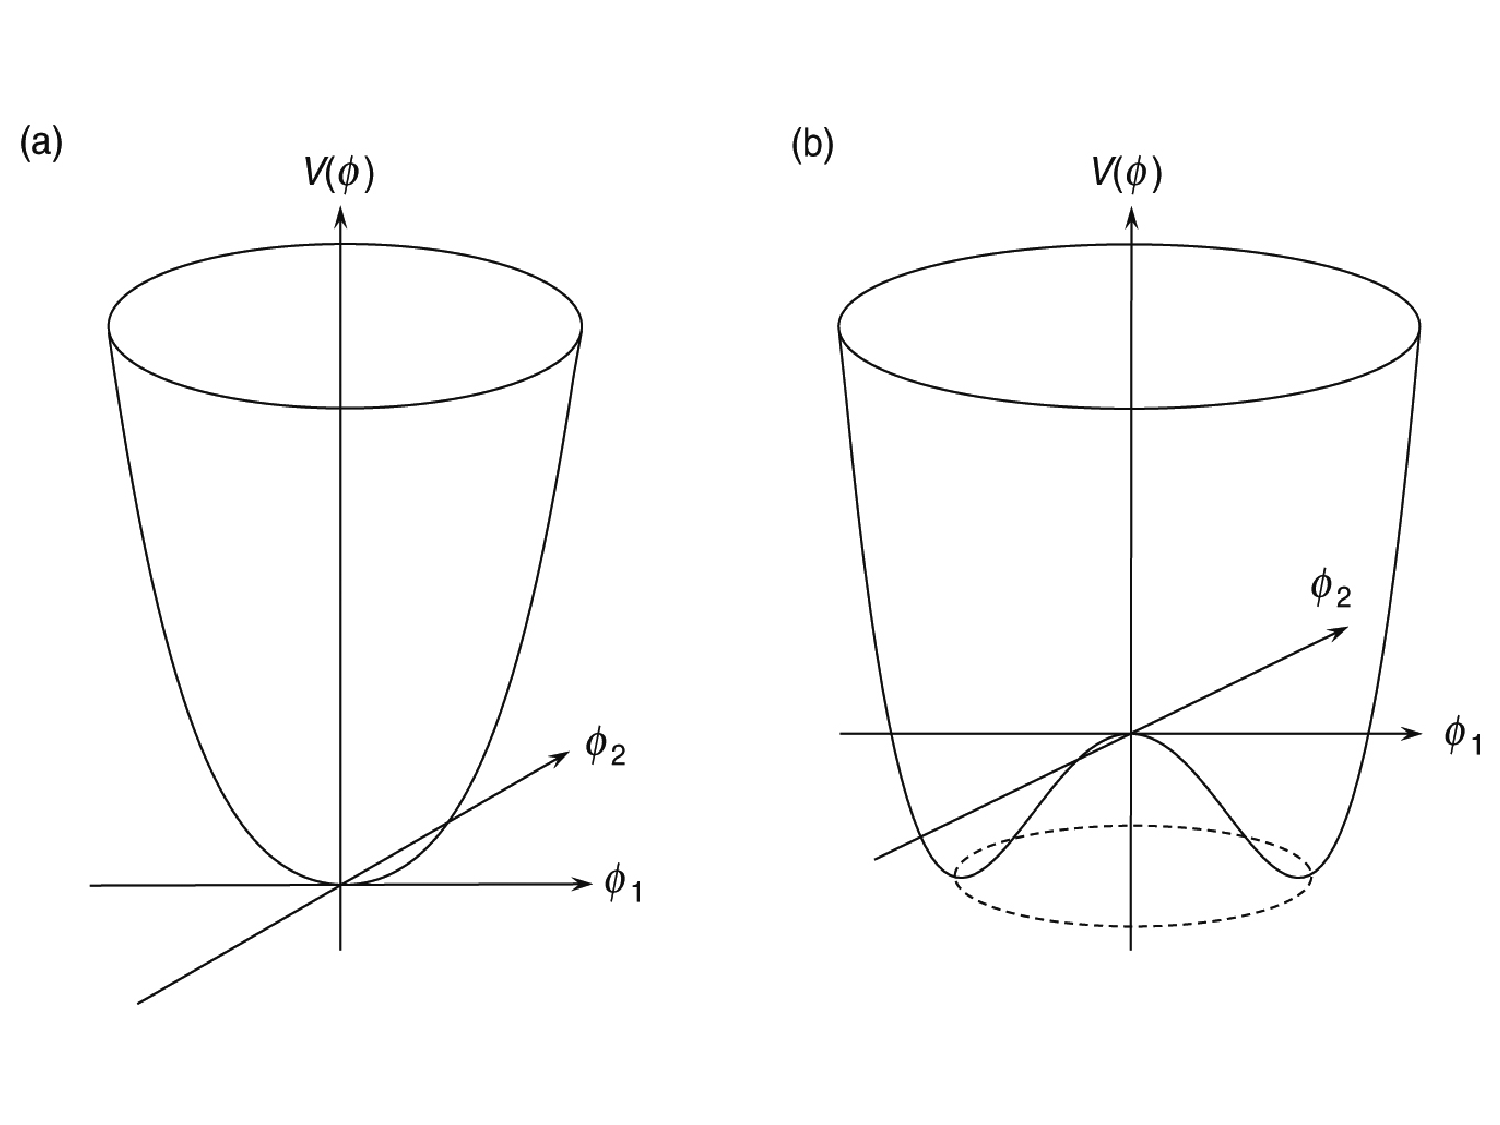
\includegraphics[width=0.8\linewidth]{figs/symm_break.pdf}
\caption{Linear sigma model potential for $N=2$. In (a) the $\phi$ field
         mass term $m^2>0$, while (b) gives this potential when
         $m^2$ is replaced by a negative parameter $-\mu^2$.
         Oscillations along the circle of minima in (b) correspond to 
         the $\pi$ field. Oscillations in the radial direction correspond
         to the $\sigma$ field. Image taken from 
         Thompson~\cite{thomson_modern_2013}.}
\label{fig:ssb}
\end{figure}

Let's try to gain some geometric intuition for this phenomenon. 
Looking at \equatref{eq:phidir}, we see that in $\phi$ space, the $\sigma$
field corresponds to oscillations of $\phi$ orthogonal to the $N-1$
dimensional hypersurface, while the massless $\pi_k$ fields
corresponds to oscillations along the hypersurface. 
An example with $N=2$ is shown in \figref{fig:ssb}. 
If we take the ground state vector~\eqref{eq:phidir} and hit it with
$\text{O}(N)$, it will be rotated somewhere else on the hypersurface.
The subgroup $\text{O}(N-1)$ hits the first $N-1$ components of the
ground state, which are all 0, thereby leaving it unchanged.
In the original $\phi^4$ theory with
$m^2>0$, the ground state vector was 0, so the $\text{O}(N)$ symmetry
was also a symmetry of the ground state. After SSB, $\text{O}(N)$ changes 
the ground state vector in general,
which is why we say the symmetry is broken. Generally any symmetry
respected by the Lagrangian but not by the ground state vector
is a broken symmetry.

In the linear sigma model, massless $\pi$ particles appeared after
SSB. This is a special example of a general result
known as Goldstone's theorem. The generated massless particles are
referred to as \index{Goldstone!boson}{\it Goldstone bosons}. 
Many light bosons can be interpreted
as approximate Goldstone bosons; as we will see in \secref{sec:cscont},
the pion can be viewed in this manner.
\begin{theorem}{Goldstone's theorem}{}
\index{Goldstone!theorem}
Consider a Lagrangian of the form
$$
  \Lagr=(\text{kinetic term for $\phi$})+
        (\text{terms independent of $\phi$})-V(\phi),
$$
where $\phi$ is the $N$-dimensional vector of real, scalar fields
$\phi_k$, and $\Lagr$ is invariant under a continuous, global
transformation of $\phi$ with generators $T^a$. Then for every
spontaneously broken generator there exists a corresponding
Goldstone boson. 
\begin{proof}
  Let $\phi_\text{min}$ be a constant field minimizing $V$. Expanding
  $V$ about this minimum we get to leading order
  $$
    V(\phi)= V(\phi_\text{min})
     +\frac{1}{2}
      (\phi-\phi_\text{min})_i(\phi-\phi_\text{min})_j\,
      \frac{\partial^2 V}{\partial\phi_i\partial\phi_j}
       \Big|_{\phi=\phi_\text{min}}.
  $$
  The differences $\phi-\phi_\text{min}$ give the new fields of the
  theory after SSB; for example in the linear sigma model this difference
  is, from \equatref{eq:phidir} and \eqref{eq:phishift},
  $$
    \phi-\phi_\text{min}=(\pi_1,...,\pi_{N-1},\sigma).
  $$
  Therefore the coefficient of the quadratic term is a symmetric matrix
  whose eigenvalues give the masses of these fields. If we can prove
  that each broken generator implies a zero eigenvalue for this matrix,
  we are done.
  The kinetic term for $\phi$ is already invariant under the global
  transformation, so if $\Lagr$ is invariant, it follows that $V$ must
  be as well. Then we can write
  $$
    V\left((\id-i\omega^aT^a)\phi\right)=V(\phi),
  $$
  where $\omega$ is some infinitesimal parameter. Expanding to linear
  order yields
  $$
    \frac{\partial V}{\partial\phi_j}(T^a\phi)_j=0.
  $$
  Differentiating the above with respect to $\phi_i$ and evaluating at
  $\phi_\text{min}$ gives
  $$
     \frac{\partial^2 V}{\partial\phi_i\partial\phi_j}
      \Big|_{\phi=\phi_\text{min}}(T^a\phi_\text{min})_j=0,
  $$
  i.e. $T^a\phi_\text{min}$ is annihilated by the mass matrix. 
  If $T^a$ is a broken generator, we have $T^a\phi_\text{min}\neq0$,
  so the above equation implies $T^a\phi_\text{min}$ is an
  eigenvector of the mass matrix with eigenvalue zero.
\end{proof}
\end{theorem}




\section{The GMOR formula}

The Gell-Mann-Oakes-Oakes-Renner (GMOR) formula~\cite{gell-mann_behavior_1968}
relates the pion mass to the masses of the up and down quarks. I think
this formula is derivable in chiral perturbation theory. The formula
takes the form
\begin{equation}
  M_\pi^2= B(m_u+m_d)+\order{m^2}.
\end{equation}
This formula directly shows that the pion mass is not simply the sum of
the valence quark masses. Moreover since you know the physical values
of $M_\pi$, $m_u$, and $m_d$, this equation can be used to crudely estimate
$M_\pi$ for unphysical light quark masses.




\section{Chiral symmetry}\label{sec:cscont}
\index{chiral symmetry}


In this section we work with a Euclidean metric. We follow
Chapter 7 of Gattringer and
Lang~\cite{gattringer_quantum_2010}.

The massless fermion action for a single flavor reads
\begin{equation}
S_F=\int\dd[4]{x}\Lagr_F=\int\dd[4]{x}\bar{\psi}\slashed{D}\psi. 
\end{equation}
We refer to $\slashed{D}$ as the {\it massless Dirac operator}. A
\index{rotation!chiral}
{\it chiral rotation}\footnote{You may notice that the sign in the exponent
is the same for both the spinor field and its conjugate field. This is a
common feature whenever a $\gamma_5$ is in the exponent. Recall that
$\bar{\psi}=\psi^\dagger\gamma_4$. The $\gamma_5$ will anticommute with
$\gamma_4$.} of the fermion fields is a transformation
mapping
\begin{equation}\label{eq:chiralRotation}
  \psi\to e^{i\alpha\gamma_5}\psi~~~~\text{and}~~~~
  \bar{\psi}\to\bar\psi e^{i\alpha\gamma_5},
\end{equation}
where $\alpha\in\R$. This is probably called a chiral rotation
because $\gamma_5$ is used to define the operators~\eqref{eq:projdef},
which project out the left-handed and right-handed components of the
fermion field according to \equatref{eq:projact}. Using identity 2 of
\propref{prp:gammatech}, we find that $\Lagr_F$ transforms under this
rotation as
\begin{equation}
  \Lagr_F\to\bar{\psi}e^{i\alpha\gamma_5}\slashed{D}e^{i\alpha\gamma_5}\psi
         =\bar{\psi}e^{i\alpha\gamma_5}e^{-i\alpha\gamma_5}\slashed{D}\psi
         =\Lagr_F,
\end{equation}
i.e. it is invariant under chiral rotations. Using
\propref{prp:projection}, one can decompose $\Lagr_F$ into its
left-handed and right-handed parts as
\begin{equation}
  \Lagr_F=\bar{\psi}_L\slashed{D}\psi_L
         +\bar{\psi}_R\slashed{D}\psi_R,
\end{equation}
and we colloquially say that the chiral components of
$\Lagr_F$ ``do not talk to each other."
If one were to include a mass term in $\Lagr_F$, it would decompose as
\begin{equation}
  m\bar{\psi}\psi=m\left(\bar{\psi}_R\psi_L+\bar{\psi}_L\psi_R\right),
\end{equation}
which mixes the chiral components, thereby breaking chiral symmetry.
\index{limit!chiral}
This is why one refers to the limit $m\to0$ as the {\it chiral limit}.




We now generalize these ideas to $N_f$ flavors of fermion. In Gattringer
and Lang eq.~(7.11), they write the fermion action as
\begin{equation}\label{eq:nfact}
  S_F=\int\dd[4]{x}\Lagr_F=\int\dd[4]{x}
         \bar{\psi}\left(\slashed{D}+M\right)\psi,
\end{equation}
where $M$ is the {\it mass matrix}\index{mass matrix}
\begin{equation}
  M~``="~\diag(m_1,m_2,...,m_{N_f})
\end{equation}
acting in flavor space. $M$ cannot be a $N_f\times N_f$ matrix, because
we have defined $\gamma^\mu$ as a $4\times4$ matrix. The only way adding
these matrices makes sense is if $M$ is a $4N_f\times4N_f$ matrix, i.e. if
\begin{equation}
  M=\left(\begin{array}{cccc}
      m_1\id_4 &          &        & \\
               & m_2\id_4 &        & \\
               &          & \ddots & \\
               &          &        & m_{N_f}\id_4
    \end{array}\right).
\end{equation}
Then $\psi$ must be a $4N_f$ vector (in the mathematical sense, not
in the Lorentz transformation sense) looking something like
\begin{equation}
  \psi=\colvec{4}{\psi_1}{\psi_2}{\vdots}{\psi_{N_f}},
\end{equation}
where each $\psi_i$ is a 4-component Dirac spinor, and presumably when
we write $\gamma^\mu$ in \equatref{eq:nfact} what we really mean is
\begin{equation}
  \gamma^\mu=\gamma^\mu\id_{N_f}
            =\left(\begin{array}{cccc}
               \gamma^\mu &            &        & \\
                          & \gamma^\mu &        & \\
                          &            & \ddots & \\
                          &            &        & \gamma^\mu
               \end{array}\right).
\end{equation}
I pray the reader forgives the notational perversion in the above equation.


In the chiral limit, the action \equatref{eq:nfact} is again invariant under
\index{rotation!axial vector}
chiral rotations, also in this context called {\it axial vector rotations},
taking the form
\begin{gather}
  \label{eq:SUNfc}
  \psi\to e^{i\alpha\gamma_5 T^a}\psi,\qquad
    \bar{\psi}\to\bar{\psi}e^{i\alpha\gamma_5 T^a}, \\
  \label{eq:U1A}
  \psi\to e^{i\alpha\gamma_5 \id}\psi,\qquad
    \bar{\psi}\to\bar{\psi}e^{i\alpha\gamma_5 \id},
\end{gather}
where the $T^a$ are the $N_f^2-1$ generators of $\SU(N_f)$,
$\id\equiv\id_{4N_f}$, and again $\alpha\in\R$.
In this limit the action is also invariant under the
\index{rotation!vector}
{\it vector rotations}
\begin{gather}
  \label{eq:SUNf}
  \psi\to e^{i\alpha T^a}\psi,\qquad
    \bar{\psi}\to\bar{\psi}e^{-i\alpha T^a}, \\
  \label{eq:U1V}
  \psi\to e^{i\alpha \id}\psi,\qquad
    \bar{\psi}\to\bar{\psi}e^{-i\alpha \id}.
\end{gather}
This invariance under the above two equations extends to the case of degenerate
masses, when $m_1=m_2=...=m_{N_f}\equiv m$, and is the familiar isospin
symmetry generalized to $N_f$ flavors. The symmetry~\eqref{eq:U1V} holds for
\index{baryon number}
arbitrary masses, and the conserved quantity is the 
{\it baryon number}\footnote{You can see why it's called baryon number: 
A baryon is made of 3
quarks, and hence has $B=1$. Anti-quarks have $B=-1$, and
mesons have $B=0$.}
\begin{equation}
    B=\frac{1}{3}(n_q-n_{\bar{q}}).
\end{equation}


Returning once again to the massless limit, the invariance of the action under
\equatref{eq:SUNfc}, \eqref{eq:U1A}, \eqref{eq:SUNf}, and \eqref{eq:U1V}
represents the global symmetry group
\begin{equation}\label{eq:SMfglobal}
  \SU(N_f)_L\times\SU(N_f)_R\times\U(1)_V\times\U(1)_A.
\end{equation}
Breaking the global symmetry group~\eqref{eq:SMfglobal} has important
implications in QCD phenomenology. For example we will show that in the
quantized, massless theory the fermion determinant changes
under~\equatref{eq:U1A}, breaking the $\U(1)_A$ symmetry explicitly. The remaining
symmetry is
\begin{equation}\label{eq:SMglobalbUA}
  \SU(N_f)_L\times\SU(N_f)_R\times\U(1)_V.
\end{equation}
If the fermion masses are degenerate, the symmetry $\SU(N_f)_L\times\SU(N_f)_R$
breaks to its subgroup $\SU(N_f)_V$. Now the remaining symmetry is
\begin{equation}
  \SU(N_f)_V\times\U(1)_V.
\end{equation}
Finally allowing non-degenerate masses breaks the symmetry further.
There remains
\begin{equation}
  \underbrace{\U(1)_V\times\U(1)_V\times...\times\U(1)_V}_\text{$N_f$ times}.
\end{equation}


The typical QCD scale is $\sim1~\text{GeV}$ (think protons, which have a
mass of about 940~MeV) so the $u$, $d$, and $s$ quarks have masses that
are relatively small (about 5~MeV, 5~MeV, and 100~MeV, respectively).
Since these masses are so close to zero on this scale, we can say that
when $N_f=2$, and partly for $N_f=3$, \equatref{eq:SMglobalbUA} is
an approximate symmetry. If the $u$ and $d$ quarks were massless, this symmetry
would be exact, and it can be argued~\cite{gattringer_quantum_2010} that
a nucleon and its negative parity partner should have the same mass.
However one finds the negative parity nucleon to have
a mass of about 1535~MeV, and this difference of about 600~MeV is too large to
be explained by the slight breaking due to the $u$ and $d$ masses. We
conclude that something else is happening. This is another example
of SSB: If quarks were massless, the pions would arise as
the Goldstone bosons of chiral SSB; hence we refer to pions as
``would-be" Goldstone bosons.


\bibliographystyle{unsrtnat}
\bibliography{bibliography}
